\documentclass[]{article}

\usepackage{pgf-pie}
\usepackage{url}
\usepackage[utf8]{inputenc}
\usepackage[T1]{fontenc}
\usepackage{amsthm}
\usepackage{qtree}

\theoremstyle{definition}
\newtheorem{ex}{Voorbeeld}[section]

% \newcounter{examplecounter}
% \newenvironment{ex2}
%   {
%     \begin{verse}
%       \refstepcounter{examplecounter}
%       (vb\arabic{examplecounter})
%       \quad
%   }
%   {
%     \end{verse}
%   }

\title{Natural Language processing for Knowledge Representation} \author{Jens
  Claes}

\newcommand{\example}[1]{\textit{``#1''}}

\begin{document}

\maketitle

\section{Inleiding}
TODO

\section{Probleemstelling}
\paragraph{} Bedrijfsprocessen worden geregeld door specificaties. Deze worden vaak geschreven in een natuurlijke taal, door een domein expert. Vervolgens worden deze specificaties vertaald naar uitvoerbare programma's. Bij deze vertaling slopen er fouten in. Bovendien zijn er vaak meerdere programma's die elk opnieuw de specificatie moeten implementeren. Zo ontstaan er niet allen inconsistenties met de specificatie, maar ook tussen de verschillende programma's onderling. Ten slotte is het moeilijk om de specificatie achteraf nog aan te passen omdat alle programma's dan aangepast moeten worden.

\paragraph{} Het antwoord van de academische wereld op deze problemen, is het
\textit{Knowledge Base Systems (KBS)}-paradigma. In dit paradigma worden de specificaties in natuurlijke taal vertaald naar specificaties in een formele taal. Deze formele specificatie wordt gebruikt in alle programma's. Zo is het niet meer mogelijk dat de programma's onderling inconsistent zijn. Ze gebruiken namelijk allemaal de formele specificatie. Daardoor is ook het aanpassen van de specificatie makkelijker. Enkel de formele specificatie moet aangepast worden, de programma's blijven hetzelfde.

\paragraph{} Het probleem met deze aanpak is dat er nog steeds een vertaling moet gebeuren van natuurlijke taal naar een formele taal. De specificatie in natuurlijke taal wordt vaak opgesteld door een domein expert die formele talen niet machtig is. De formele specificatie wordt dan weer opgesteld door een KBS expert. Deze persoon kent formele talen maar heeft een beperkte kennis van het domein. Door deze mismatch van kennis, is de feedback loop tussen de twee experten beperkt. Het is dus nog steeds mogelijk dat er fouten sluipen in de vertaling.

\paragraph{} De vraag rijst dus of we een formele taal kunnen ontwerpen die toegankelijk is voor domein experten, rijk genoeg is voor praktische problemen en toepasbaar is binnen het KBS paradigma.

\paragraph{} Deze thesis onderzoekt of een formele natuurlijke taal het antwoord is op die vraag. Natuurlijke taal wordt immers al gebruikt bij het opstellen van de specificatie. Figuur \ref{fig:natural-language-use} toont het gebruik van natuurlijke taal in vereistenanalyse in 1999. Slechts 5 procent werd toen in een formele taal opgesteld. 16 procent werd in gestructureerde natuurlijke taal opgesteld. Dit wil zeggen dat de specificatie in een natuurlijke taal is opgesteld maar slechts een beperkt aantal zinsconstructies zijn toegestaan, om de leesbaarheid te verhogen.

\begin{figure}
  \label{fig:natural-language-use}
  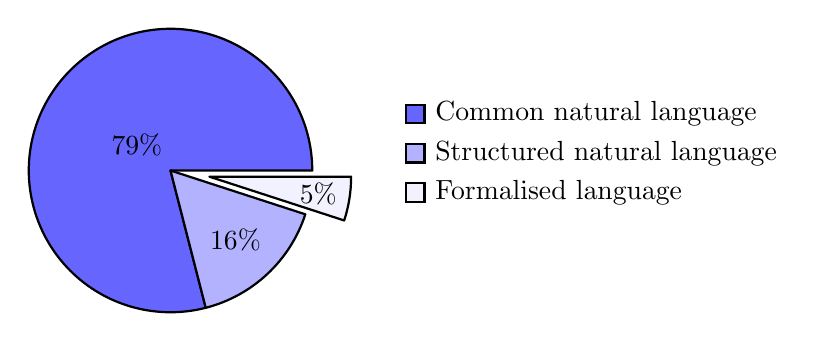
\begin{tikzpicture}
      \pie[text = legend, radius = 1.8, explode = {0, 0, 0.5}, color = {blue!60, blue!30, blue!5}]{79/Common natural language, 16/Structured natural language, 5/Formalised language}
  \end{tikzpicture}
  \caption{Gebruik van natuurlijke taal in vereistenanalyse in 1999 (van figuur 5 in \cite{Luisa2004})}
\end{figure}

\paragraph{} In deze thesis ontwerpen we een nieuwe gestructureerde natuurlijke taal (vanaf nu CNL genoemd naar de Engelse term Controlled Natural Language). Het doel van deze taal is dat ze leesbaar is voor de domein expert, de KBS expert en computers. Zo kan een programma de formele specificatie opstellen vanuit de specificatie in de natuurlijke taal. Er is dan nog maar 1 bron van waarheidwaaruit alles geregeld wordt. Inconsistenties zijn niet meer mogelijk. Bovendien kan men nog steeds makkelijk de specificatie aanpassen.

\section{Literatuurstudie}
In het verleden zijn er al meerdere CNL's gemaakt. Sommige zijn ontwerpen om de leesbaarheid van de specificaties te verhogen en hebben geen formele semantiek. Kuhn heeft een classificatieschema ontwerpen voor al deze CNL's \cite{Kuhn2014} genaamd PENS: Precision (hoe ambigu/formeel is de taal), Expressivity (welke problemen kunnen we uitdrukken), Naturalness (hoe vlot leest de taal), Simplicity (hoe simpel is de taal). In dezelfde paper lijst Kuhn ook een heleboel CNL's op met hun geschiedenis en nut alsook hun classificatie volgens het PENS-schema.

Teksten in natuurlijke taal omvormen tot formele modellen is al gebeurd in verschillende domeinen: vereistenanalyse, regelgebaseerde paradigma's maar ook binnen het domein van de computationele linguïstiek. Deze sectie geeft een kort overzicht van wat er al gebeurd is in deze domeinen. Voor een completer overzicht van CNL's, verwijzen we naar \cite{Kuhn2014}.

\subsection{Vereistenanalyse}
\paragraph{Circe} De tool Circe\cite{Ambriola1997} wordt gebruikt in vereistenanalyse. De gebruiker moet een vocabularium, een set van substitutieregels en een specificatie in natuurlijke aanleveren. De tool probeert dan steeds de beste regel te vinden om zo de tekst geleidelijk aan te transformeren naar een formeel model. Het grote voordeel van de methode is dat er regelsets bestaan voor meerdere soorten modellen: data flow modellen, entity-relationship modellen, ...

Verder is het in Circe mogelijk om in het vocabularium woorden te taggen. De regels kunnen hier dan gebruik van maken om te bepalen of ze van toepassing zijn op bepaalde zinnen. Op die manier introduceert Circe types in het vocabularium.

Een voorbeeld (uit \cite{Ambriola1997}): \example{bron/UIT STUURT data/INFO NAAR doel/IN}. De woorden \example{stuurt} en \example{naar} liggen vast in de regelset. De andere 3 woorden komen uit het vocabularium. Deze moeten een bepaalde tag hebben om te matchen met de regel.

Circe is geen CNL. Zinnen die niet matchen met een substitutieregel worden ook niet omgezet in een formeel model.

\subsection{Business rules}
Ook binnen het paradigma van business rules spelen zowel natuurlijke talen als formele talen een grote rol. SBVR Structured English (SBVR-SE)\cite{Levy2013} en RuleSpeak\cite{Ross2009a} zijn 2 CNL's die proberen om ambiguïteit in de natuurlijke taal te verminderen. Deze talen focussen echter vooral op het menselijke aspect. Het doel van deze talen is om ambiguïteit uit de specificatie te halen en niet zozeer om automatisch natuurlijke taal om te zetten naar een formele voorstelling. RuleCNL\cite{Njonko2014} heeft wel dit doel.

RuleCNL splitst de specificatie op in twee delen: een vocabularium en de regels zelf. Het vocabularium bestaat uit substantieven en werkwoorden alsook hoe deze in verhouding staan tot elkaar. Bijvoorbeeld \example{Auto heeft wiel} geeft aan dat er een relatie kan bestaan tussen een auto en een wiel. Voor de regels zelf bestaat er een contextvrije grammatica waaraan de zinnen moeten voldoen.

Om de gebruikers te helpen bij het schrijven van de zinnen in RuleCNL, is er een plugin voor de Eclipse IDE die automatisch zinnen kan aanvullen en de structuur van bestaande zinnen aangeeft door het kleuren ervan. Bovendien is er een visuele representatie van het domein om de gebruiker te helpen bij het schrijven van het vocabularium.

\subsection{Computationele linguïstiek} Binnen het domein van de computationele linguïstiek zijn er al 2 belangrijke CNL's opgesteld die vertaald kunnen worden naar formele modellen: Attempto Controlled English (ACE) en Processable English (PENG). Beiden talen lijken op elkaar en hebben gelijkaardige tools om mee te werken. In de rest van deze sectie volgt eerst een bespreking van ACE. Daarna bespreken we PENG. Hierbij ligt de nadruk op de gelijkenissen en verschillen met ACE. We sluiten af met een beschrijving van hoe deze twee talen geïmplementeerd zijn.

\subsubsection{Attempto Controlled English (ACE)}
\paragraph{} Attempto Controlled English\cite{Fuchs2008} is een gestructureerde taal voor kennisrepresentatie. Het is een subset van Engels die naar een subset van eerste-orde-logica vertaald. Het is echter wel een formele taal: elke zin in ACE heeft slechts één betekenis, ook al is de Engelse zin ambigu. Om de juiste betekenis te kennen, kan men gebruik maken van de parafraseertool van ACE. Deze tool zet de interne representatie terug om naar één of meerdere zinnen in ACE. Op die manier kan men niet alleen de betekenis van de zin leren, maar ook de taal zelf.

ACE is een general purpose CNL: Het bevat een ingebouwd vocabularium. De gebruiker moet dus zelf geen vocabularium opstellen en kan direct beginnen met het schrijven van de specificatie. Het nadeel aan deze aanpak is dat ACE dus ook geen domeinkennis kan gebruiken voor het analyseren van de zinnen. Sommige constructies moeten daarom met een koppelteken geschreven worden. Zo wordt er in \cite{ACEConstructionRules} het voorbeeld gegeven van \example{A student is interested-in a course} en \example{A student is interested in a classroom}.

Op die manier probeert ACE sommige ambiguïteiten op te lossen. Een gelijkaardige truk wordt bijvoorbeeld ook gebruikt om de voorrang van \example{en} en \example{of} op te lossen. Standaard heeft \example{en} voorrang. Maar als de \example{en} voorafgegaan wordt door een komma, dan heeft \example{of} voorrang. \cite{ACEConstructionRules} geeft het voorbeeld \example{A client \{enters a red card or enters a blue card\}, and enters a code.}

In andere gevallen kiest ACE gewoon hoe de zin geïnterpreteerd moet worden op basis van een set van \textit{interpration rules}. Zo slaat de \example{manually} in \example{A customer who {enters a card manually} types a code.}\cite{ACEConstructionRules} op \example{enters} en niet op \example{types} omdat een bijwoord bij voorkeur achter het werkwoord staat.

Één van de sterke punten van ACE is het oplossen van anaforische referenties (referenties naar woorden eerder in de zin of naar woorden van vorige zinnen). De invoertekst wordt namelijk als één geheel vertaald. Daardoor is het niet nodig om lange zinnen met veel bijzinnen te schrijven. Men kan zo'n zinnen namelijk opbreken in een aantal kortere zinnen. Zo kan \example{A customer inserts a card that carries a code.} geschreven worden als \example{A card carries a code. A customer inserts the card.}\cite{Fuchs2008}. Op deze manier blijft de specificatie leesbaar.

\paragraph{} Origineel was ACE bedoeld voor het opstellen van specificaties voor software. Ondertussen kent de taal al meerdere toepassingen, in verschillende domeinen. Er zijn ook meerdere tools die overweg kunnen met ACE als input.

Zo is er de Attempto Parsing Engine APE die ACE zinnen omzet naar Discourse Representation Structures (DRS). Deze variant op eerste-orde-logica wordt vooral gebruikt voor de coreferentie-analyse. Met behulp van de DRS-structuren is het namelijk makkelijker om te acherhalen naar welke woordgroep de anaforische referenties verwijzen. APE geeft ook een parafrasering van de invoertekst. Zodat de gebruiker kan controleren of de tool de tekst op de juiste manier leest. Bovendien kan APE waarschuwingen geven bij mogelijke problemen. Bijvoorbeeld het gebruik van een anaforische referentie (zoals een bepaald lidwoord) zonder een antecedent waarnaar deze anafoor kan verwijzen.

Verder is er ook de Attempto Reasoner RACE. Deze tool kan controleren of een specificatie consistent is met zichzelf. De tool zal dan zeggen welke zinnen met elkaar in conflict zijn. Op die manier weet de gebruiker dat er een fout is en waar deze zich ongeveer bevindt. De tool kan ook vragen in natuurlijke taal beantwoorden. RACE antwoordt niet alleen op de vraag maar geeft ook de zinnen die nodig zijn om te bewijzen dat het gegeven antwoord juist is. Ten slotte kan RACE bewijzen of een bepaalde zin het logische gevolg is van de specificatie. Op die manier kan de gebruiker testen of de specificatie correct is.

APE en RACE zijn de twee belangrijkste tools. Er zijn er echter nog veel meer. Zo is er de ACE View Protégé plug-in. Dit is een plugin die de vertaling tussen Web Ontology Language (OWL) en ACE doet binnen de Protégé-omgeving (een editor voor het maken van ontologiën). Op die manier ziet de gebruiker enkel ACE zinnen en hoeft dus de formele OWL taal niet te kennen om met bestaande modellen om te gaan of om nieuwe modellen te maken. Ten slotte is er ook nog AceRules. Hiermee kan de gebruiker de zinnen die geïmpliceerd worden door de specificatie te weten komen.

Over het algemeen is ACE een zeer uitgebreide taal. Veel Engelse zinnen zijn ook geldige ACE zinnen, echter niet allemaal. Dit zorgt ervoor dat het soms niet duidelijk is welke zinnen geldig zijn en welke niet. Volgens \cite{Fuchs2008} heeft een gebruiker 2 dagen nodig om de taal te leren.

\subsubsection{Processable English (PENG)}
\paragraph{} Andere talen zoals PENG\cite{Schwitter2002} zijn makkelijker om te leren. PENG is ook een CNL die vertaald naar DRS-structuren. In tegenstelling tot ACE bevat PENG geen groot ingebouwd lexicon. De gebruiker moet zelf de woorden aanbrengen die gebruikt worden. De gebruiker kan dit doen tijdens het bewerken en moet dus niet op voorhand aangeven wat het lexicon is. De categorieën voor deze domeinspecifieke woorden zijn: zelfstandig naamwoord, bijvoeglijk naamwoord, werkwoord en bijwoord. PENG biedt ook de mogelijkheid om synoniemen of afkortingen te introduceren. Op die manier kan de specificatie vlotter gemaakt worden. Naast de domeinspecifieke woorden kent PENG ook een aantal functionele woorden die ingebakken zitten in de taal. Deze woorden helpen PENG om de zinsconstructies te herkennen.

Net zoals ACE kent PENG het principe van constructieregels en interpretatieregels. De constructieregels bepalen welke zinnen deel zijn van de taal. Bij PENG zijn deze regels eenvoudiger omdat de taal zeer simpel gehouden is. Op die manier willen ze het makkelijker maken om zinnen te maken in de taal. Over het algemeen lijken de constructieregels van PENG en ACE veel op elkaar.

De interpretatieregels bepalen hoe de zin vertaald wordt naar logica. Zo is er een interpretatieregel voor hoe anaforische referenties opgelost worden. Deze regel is gelijkaardig in ACE en PENG. Andere regels bepalen welke functiewoorden sterker binden. Zowel ACE als PENG gebruiken hiervoor dezelfde volgorde als in eerste-orde-logica. ACE staat wel uitzonderingen toe door het toevoegen van komma's. PENG houdt de taal simpel en staat dit niet toe.

\paragraph{} PENG is makkelijker om te leren dan ACE omwille van ECOLE\cite{Schwitter2003}. Deze tool kan suggesties geven over de woordcategorieën die kunnen volgen op een bepaalde zin. Zo geeft \cite{Schwitter2003} het voorbeeld van \example{Een} dat gevolgd kan worden door een \texttt{adjectief} of een \texttt{substantief}. Indien de gebruiker de woordcategorie niet kent, kan hij doorklikken op die categorie voor een aantal concrete mogelijkheden. Op die manier moet de gebruiker enkel de woordcategorieën leren en niet de geldige zinsconstructies.

Naast de suggestietool bevat PENG, net zoals ACE, ook een parafraseertool. Deze tool herschrijft de invoer zodat het duidelijker is hoe PENG de zin begrepen heeft. Anaforische referenties worden bijvoorbeeld omgezet in de noun phrase naarwaar ze verwijzen.

Net zoals in ACE is het ook in PENG mogelijk om te controleren of een specificatie consistent is\cite{Schwitter2004b}. Daarnaast is het mogelijk om te controleren op redundantie. Indien een zin al door een andere zin geïmpliceerd wordt, hoeft deze niet expliciet deel uit te maken van de specificatie. Op die manier kan de specificatie kort gehouden worden, wat de leesbaarheid verhoogd.

Naast de general purpose CNL bevat PENG ook een subset specifiek voor het semantische web: PENG-D\cite{Schwitter2004}. Deze subset is wel beslisbaar en kan vertaald worden naar description logic, een subset van eerste-orde-logica. PENG-D kan dus gezien worden als het alternatief voor de ACE View Protégé plug-in.
\cite{Schwitter2006} vermeldt drie klassieke manieren van voorstellen van een ontologie (N-Triples, RDF/XML en OWL Abstract) en toont dan verder aan dat PENG een vierde manier is om hetzelfde voor te stellen. De paper toont dit aan door verschillende constructies uit OWL te mappen op zinnen in PENG. Het grote voordeel van PENG t.o.v. de andere voorstellingswijzen is dat PENG ook leesbaar en begrijpbaar is voor de mens.

\subsubsection{Implementatie}
\paragraph{} Zowel ACE als PENG zijn geïmplementeerd in prolog met behulp van Definite Clause Grammars (DCG) en feature structures voor het omzetten van de natuurlijke taal naar DRS-structuren\cite{Fuchs2008, Schwitter2006}.

\paragraph{DCG} Definite Clause Grammars\cite{Pereira1980} zitten vaak ingebakken in logische talen. Deze grammatica's zijn een uitbreiding van contextvrije grammatica's. \cite{Pereira1980} geeft 3 voorbeelden van hoe DCG's kunnen helpen bij het parsen van natuurlijke talen:

\begin{enumerate}
  \item De woordvorm kan afhankelijk gemaakt worden van de context waarin deze verschijnt. Zo kan men eisen dat een werkwoord in de juiste vervoeging voorkomt.
  \item Tijdens het parsen kan men een boom opbouwen die de semantiek van de zin moet vatten. Deze boom hoeft niet isomorf te zijn met de structuur van de grammatica.
  \item Het is mogelijk om prolog code toe te voegen die extra restricties oplegt aan de grammatica.
\end{enumerate}

\begin{ex}
  Een voorbeeld van een DCG grammatica is:
  \begin{quote}
    \texttt{s ---> np, vp.} \\
    \texttt{np ---> [ik].} \\
    \texttt{np ---> [hem].} \\
    \texttt{vp ---> v, np.} \\
    \texttt{v ---> [zie].}
  \end{quote}
\end{ex} 
\texttt{s} is het startsymbool en staat voor \texttt{sentence}. \texttt{np} staat voor \texttt{noun phrase}, \texttt{vp} voor \texttt{verb phrase} en \texttt{v} voor \texttt{verb}. We gebruiken de Engelse namen voor gelijkaardigheid met de literatuur. Deze grammatica zegt dat een zin bestaat uit een noun phrase gevold door een verb phrase. Een verb phrase is dan weer een werkwoord gevolgd door een noun phrase.

De zin \example{ik zie hem} is onderdeel van deze taal. Maar ook de zin \example{ik zie ik} is deel van de taal. Om dit op te lossen kunnen we argumenten meegeven aan de niet-terminaal \texttt{np}.

\begin{ex}
  \label{ex:nom-acc-features}
  Deze verbeterde grammatica houdt rekening met welke woordvorm kan voorkomen in welke context.
  \begin{quote}
    \texttt{s ---> np(nom), vp.} \\
    \texttt{np(nom) ---> [ik].} \\
    \texttt{np(acc) ---> [hem].} \\
    \texttt{vp ---> v, np(acc).} \\
    \texttt{v ---> [zie].} \\
  \end{quote}
\end{ex} 

De \texttt{nom} en \texttt{acc} slaan hier op nominatief en accusatief. Ze geven aan in welke functie de noun phrases gebruikt mogen worden.

\begin{ex} Het is ook mogelijk om een boom op te bouwen tijdens het parsen:
  \begin{quote}
    \texttt{s(s(VP, NP)) ---> np(NP, nom), vp(VP).} \\
    \texttt{np(np(ik), nom) ---> [ik].} \\
    \texttt{np(np(hem), acc) ---> [hem].} \\
    \texttt{vp(vp(Verb, NP)) ---> v(Verb), np(NP, acc).} \\
    \texttt{v(zie) ---> [zie].}
  \end{quote}
\end{ex} 

Bij het parsen van \example{ik zie hem} krijgen we nu volgende boom:

\Tree[.s
         [.vp \textit{zie}
              [.np \textit{hem} ]]
         [.np [ \textit{ik} ]]]

Merk op dat de \texttt{vp}-tak voor de \texttt{np}-tak komt in onze boom. Dit is om aan te tonen dat de boom niet per se de structuur van de grammatica moet volgen.

\begin{ex} Ten slotte is het mogelijk om prolog code uit te voeren in de grammatica door deze prolog goals tussen accolades te plaatsen.
  \begin{quote}
    \texttt{expression(X) ---> factor(X).} \\
    \texttt{expression(X) ---> term(X).} \\

    \texttt{factor(X) ---> numeral(X).} \\
    \texttt{factor(X) ---> numberal(A), [*], factor(B), \{X is A * B\}.} \\
    \texttt{term(X) ---> factor(A), [+], expression(B), \{X is A + B\}.} \\

    \texttt{numeral(X) ---> [X], \{number(X)\}.} \\
  \end{quote}
\end{ex} 

Bovenstaande grammatica kan simpele wiskunde expressies omvormen tot de wiskundige waarde. Zo wordt \texttt{2 + 4 * 5} omgevormd tot \texttt{X = 22} volgens volgende boom:

\Tree[.expression(22)
        [.term(22) [.factor(2) [.number(2) 2 ]]
                   +
                   [.expression(20) [.factor(20) [.number(4) 4 ] * [.factor(5) [.number(5) 5 ]]]]]]

De grammatica is als volgt opgebouwd: Een expressie is ofwel een factor ofwel een term. De waarde van de expressie komt overeen met de waarde van de factor of de term.

Een factor is ofwel een getal, ofwel een vermenigvuldiging van een getal met een factor. In het laatste geval is de waarde van de factor gelijk aan de vermenigvuldiging van de waardes van de 2 subexpressies.
De uitdrukking voor een term is gelijkaardig aan die van een factor.

Ten slotte definiëren we een getal als een terminaal maar daarbij testen we nog eens of de waarde een getal is volgens prolog. \example{two + four * five} is dus geen geldige uitdrukking.

Merk op dat een factor niet gedefinieerd wordt als de vermenigvuldiging van 2 factoren. DCG's worden namelijk net als prolog top-down en van links naar rechts ``uitgevoerd''. Het is dus verboden om links recursieve regels te hebben in de grammatica want deze leiden tot een oneindige lus. Gelukkig is het altijd mogelijk om een links recursieve grammatica om te vormen tot een normale grammatica.

\paragraph{} DCG's zonder prolog code, zijn zeer declaratief: Men kan ze als object gaan gebruiken en niet langer enkel als parser/generator. Op die manier kan men ook een chart parser schrijven voor deze grammatica's. Dit is wat PENG doet in ECOLE\cite{Schwitter2003} en ACE gebruikt in AceWiki\cite{Kuhn2008}, een subset van ACE voor semantische wiki's. Een chart parser is niet alleen sneller, het is ook makkelijk om te voorspellen wat er nog kan volgen. Op die manier kan men een editor maken die voorspelt welke woordcategorie moet volgen. Maar het is ook mogelijk om in een volledige zin aan te duiden waarom die zin ongeldig is. Bijvoorbeeld in de zin \example{zag haar}, kan men zeggen \texttt{Onverwacht werkwoord ``zag''. Een onderwerp (noun phrase) werd verwacht}. \cite{Kuhn2008} legt in detail uit hoe zo'n chart parser gemaakt kan worden.

Wanneer DCG's als declaratieve definitie van een grammatica worden gezien en de semantiek van de uitvoering wegvalt, is het wel mogelijk om links recursieve grammatica's toe te laten. De chart parser kan hier namelijk rekening mee houden.

\paragraph{Feature structures} Naast DCG's wordt er in ACE en PENG ook gebruikt gemaakt van feature structures\cite{Shieber2003}. Een feature structure is een geavanceerde parse tree die vooral binnen de (computationele) linguïstiek gebruikt worden. Ze verschillen van een parse tree doordat ze een gerichte acyclische graaf zijn i.p.v. een boom. Bovendien hebben alle kinderen namen en maakt de volgorde niet uit. Men kan ze dus zien als een hashmap-achtige datastructuur waarbij de waarden ook terug een hash-map kunnen zijn maar er geen cylci zijn toegestaan. De grammatica's die gebruik maken van feature structures, gebruiken unificatie voor het samenvoegen van meerdere structuren. Niet alle features moeten namelijk een waarde toegekend krijgen. Zo kan een eigennaam voorkomen als onderwerp en als lijdend voorwerp (en heeft dus geen waarde voor de feature \texttt{naamval}). Terwijl \example{ik} enkel als onderwerp kan voorkomen (en dus wel een waarde heeft voor die feature).

\paragraph{} Binnen ACE en PENG zorgen de feature structures voor de syntactische correctheid van de zinnen in de gast taal, het Engels. Via unificatie kan men namelijk testen of een bepaalde woordgroep voldoet aan de voorwaarden van de context. Deze structuren bevatten bijvoorbeeld informatie over het getal van het onderwerp en van het werkwoord. Enkel wanneer deze 2 unificeren, is de zin geldig. Op die manier zijn zinnen die in ACE en/of PENG geldig zijn, ook geldig in het Engels. Dit is gelijkaardig aan de rol van \texttt{nom} en de \texttt{acc} in voorbeeld \ref{ex:nom-acc-features}.

\paragraph{} Zoals \cite{Shieber2003} aanhaalt, verschillen prolog termen van feature structures enkel doordat in prolog de volgorde en de ariteit wel een rol speelt. De \textit{namen} van de features in prolog zijn dus de index in de term. En alle features die mogelijk zijn, moeten voorkomen in de term, eventueel ongebonden. Daarom is het handiger om feature structures te gebruiken. Zo hoeft men niet alle voorkomens van een structure aan te passen voor het toevoegen van een argument. Bovendien moet men niet te onthouden op welke positie welk argument voorkomt. Qua expressiviteit zijn feature structures echter gelijkwaardig aan DCG's.

\paragraph{} Feature structuren zijn handig om de explosie van grammatica regels te voorkomen.
\begin{ex}  Een voorbeeld uit \cite{FeatureStructuresExplosion}:
  \label{ex:explosion}
  \begin{quote}
    \texttt{s ---> np\_{singular}, vp\_{singular}.} \\
    \texttt{s ---> np\_{plural}, vp\_{plural}.} \\
    \texttt{np ---> np\_{singular}.} \\
    \texttt{np ---> np\_{plural}.} \\
    \texttt{np\_{singular} ---> det, n\_{singular}.} \\
    \texttt{np\_{plural} ---> det, n\_{plural}.} \\
    \texttt{vp\_{singular} ---> intransitive\_verb\_{singular}.} \\
    \texttt{vp\_{singular} ---> transitive\_verb\_{singular}, np.} \\
    \texttt{vp\_{plural} ---> intransitive\_verb\_{plural}.} \\
    \texttt{vp\_{plural} ---> transitive\_verb\_{plural}, np.} \\
  \end{quote}
\end{ex} 
Hierbij staat de \texttt{n} voor zelfstandig naamwoord (noun) en \texttt{det} voor lidwoord (determiner). Deze grammatica can veel korter gemaakt worden door gebruik te maken van feature structures:

\begin{ex}  Een equivalente grammatica aan voorbeeld \ref{ex:explosion}
  \begin{quote}
    \texttt{s ---> np(FS), vp(FS).} \\
    \texttt{np(FS) ---> det, n(FS).} \\
    \texttt{vp(FS) ---> intransitive\_verb(FS).} \\
    \texttt{vp(FS) ---> transitive\_verb(FS), np(\_).} \\
  \end{quote}
\end{ex} 

Door gebruik te maken van feature structures is de grammatica simpeler en leesbaarder. Bovendien hoeft het concept dat een zin bestaat uit een noun phrase gevolgd door een verb phrase maar één keer te worden uitgedrukt. De featurestructures zorgen voor de overeenkomst in getal tussen onderwerp en werkwoord.

\paragraph{DRS} Naast feature structures maken ACE en PENG ook gebruik van Discourse Representation Structures. Deze structuren kunnen vertaald worden naar eerste-orde-logica. Ze zijn een onderdeel van Discourse Representation Theory. Dit is een taalkundig framework om de semantiek van natuurlijke taal te begrijpen. Eén van de sterke punten van DRS-structuren is het oplossen van coreferenties. \cite{Fuchs2008drs} bevat meer informatie over hoe DRS-structuren gebruikt worden binnen ACE.

\paragraph{Conclusie} DCG's is een uitbreiding op contextvrije grammatica's uit de wereld van logisch programmeren. Feature structures en Discourse Representation Structures zijn concepten uit de linguïstiek. Ze worden gebruikt om de natuurlijke taal en haar semantiek te modelleren. Zo helpen feature structures om een explosie van het aantal grammatica regels te voorkomen. Discourse Representation Structures worden dan weer vooral gebruikt om de coreferentie-analyse te vergemakkelijken. Beiden concepten passen mooi binnen ACE en PENG omdat deze talen ook ontstaan zijn in het vakgebied van computationele linguïstiek.

% TODO: evaluation CNL
% TODO: computer linguistic vs computer science!!!

% \subsection{Interessante papers} */
% \subsubsection{Done} */
% \begin{enumerate} */
%   \item ACE\cite{Fuchs2008} (\cite{Fuchs}, Master Thesis\cite{Dellis2010}) */
%   \item PENG\cite{Schwitter2002, Schwitter2004b, Schwitter2003, Schwitter2006}, (PENG Light\cite{Schwitter2008, White2009}), PENG D\cite{Schwitter2004}, ook van Schwitter:\cite{Schwitter2005}  */
%   \item Writing support for CNL's\cite{Kuhn2008}  */
%   \item Overzicht + classificatie\cite{Kuhn2014} */
%   \item RuleSpeak\cite{Ross2009a, Ross2013, Ross2013a, Ross2009}
%   \item RuleCNL\cite{Njonko2014}
%   \item SBVR\cite{Spreeuwenberg2010, Levy2013}
% \end{enumerate} */

% \subsubsection{Todo}
% \begin{enumerate}
%   \item Evaluation CNL\cite{Kuhn2010}
%   \item ------------------------------------------------------------
%   \item A principled approach to CNL's\cite{Kuhn2013}: linguistic
%   \item Model checking\cite{Flake2002, Konrad2005, Nelken, Jak2008}
%   \item Lijst van ambiguïteiten \cite{Berry2003}
%   \item CELT\cite{Pease2010, Dellis2010}
% \end{enumerate}

\section{Planning}
Momenteel kan ik al zinnen vertalen naar eerste-orde-logica. Hier zitten wel nog een aantal kleine foutjes in.
Gedurende de blok- en examenperiode plan ik geen thesiswerk in. In februari wil ik het vocabularium formaliseren en gebruiken bij het parsen van zinnen voor de theorie. Ik wil het vocabularium dan ook uit natuurlijke taal kunnen afleiden. In maart wil ik verdere uitbreidingen van de taal bekijken die de formele expressiviteit verhogen (definities, aritmetiek, aggregaten, ...). In april wil ik al beginnen schrijven aan de tekst. Verder wil ik dan een groter probleem uitdrukken in de nieuwe natuurlijke taal om te testen hoe expressief ze is op formeel vlak en hoe leesbaar de specificatie is voor reële problemen. In mei plan ik enkel nog te schrijven aan mijn thesis.

\pagebreak
\section{Referenties}
\bibliographystyle{unsrt}
\bibliography{tekst}

\end{document}


% LocalWords: KBS Systems Knowledge programma's
